\section*{Backtesting Results}

The backtesting results for the Value-at-Risk (VaR) models are summarized below.

For the Parametric Normal model, a total of 77 violations were recorded, corresponding to a violation rate of 1.85\%. The Kupiec test statistic was 24.3929 with a p-value of 0.0000. The Christoffersen independence test yielded a value of 15.6251 (p-value: 0.0001). The joint likelihood ratio test resulted in a statistic of 40.0180 with a p-value of 0.0000.

\begin{figure}[H]
    \centering
    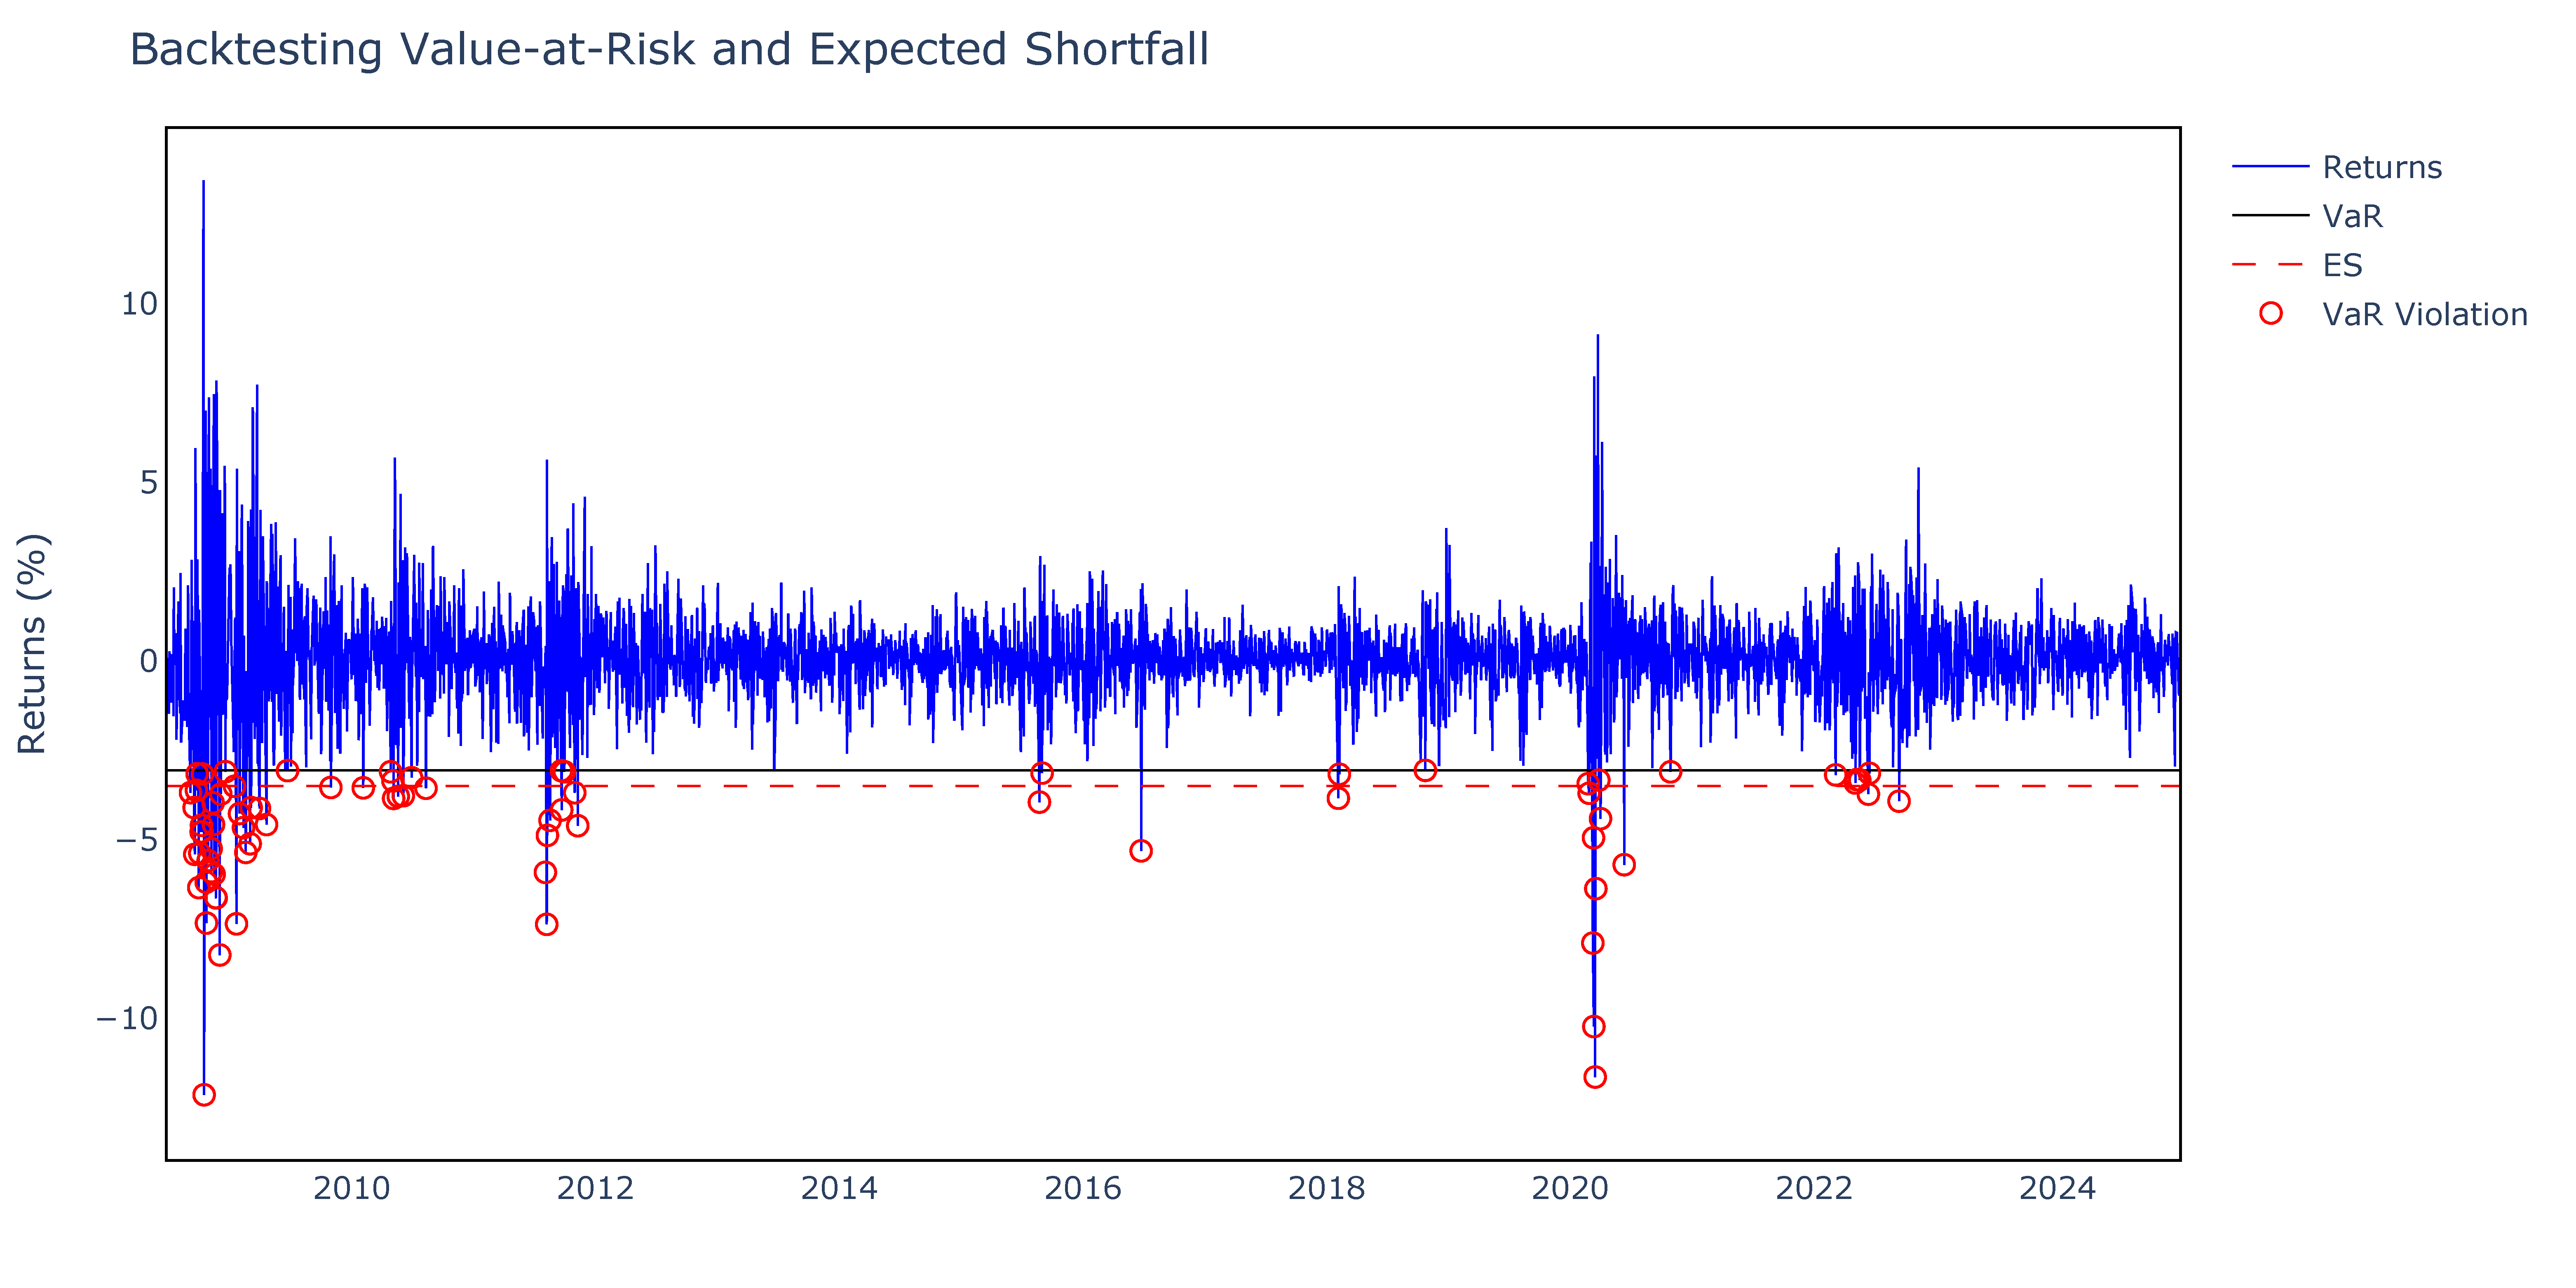
\includegraphics[width=0.8\textwidth]{figures/parametric_backtest.pdf}
    \caption{Backtest of Parametric Normal VaR}
\end{figure}

For the Historical Simulation model, 42 violations occurred, corresponding to a violation rate of 1.01\%. The Kupiec test returned a value of 0.0047 (p-value: 0.9454), and the Christoffersen test statistic was 22.2057 (p-value: 0.0000). The joint test statistic was 22.2104 with a p-value of 0.0000.

\begin{figure}[H]
    \centering
    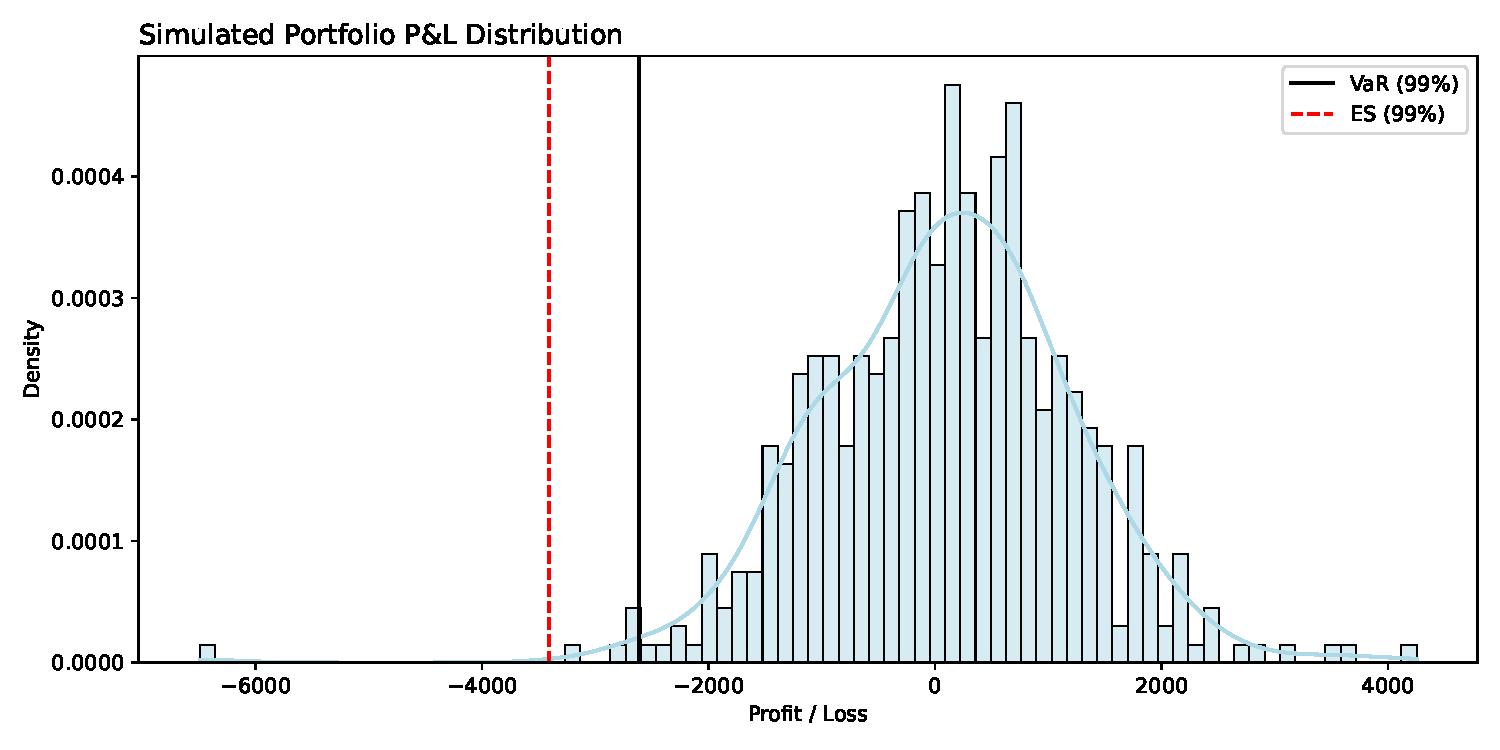
\includegraphics[width=0.8\textwidth]{figures/historical_simulation.pdf}
    \caption{Backtest of Historical Simulation VaR}
\end{figure}

In the Monte Carlo simulation model, the estimated 1-day VaR at 99\% confidence was CHF 2,516.22, while the corresponding Expected Shortfall was CHF 2,875.99.

\begin{figure}[H]
    \centering
    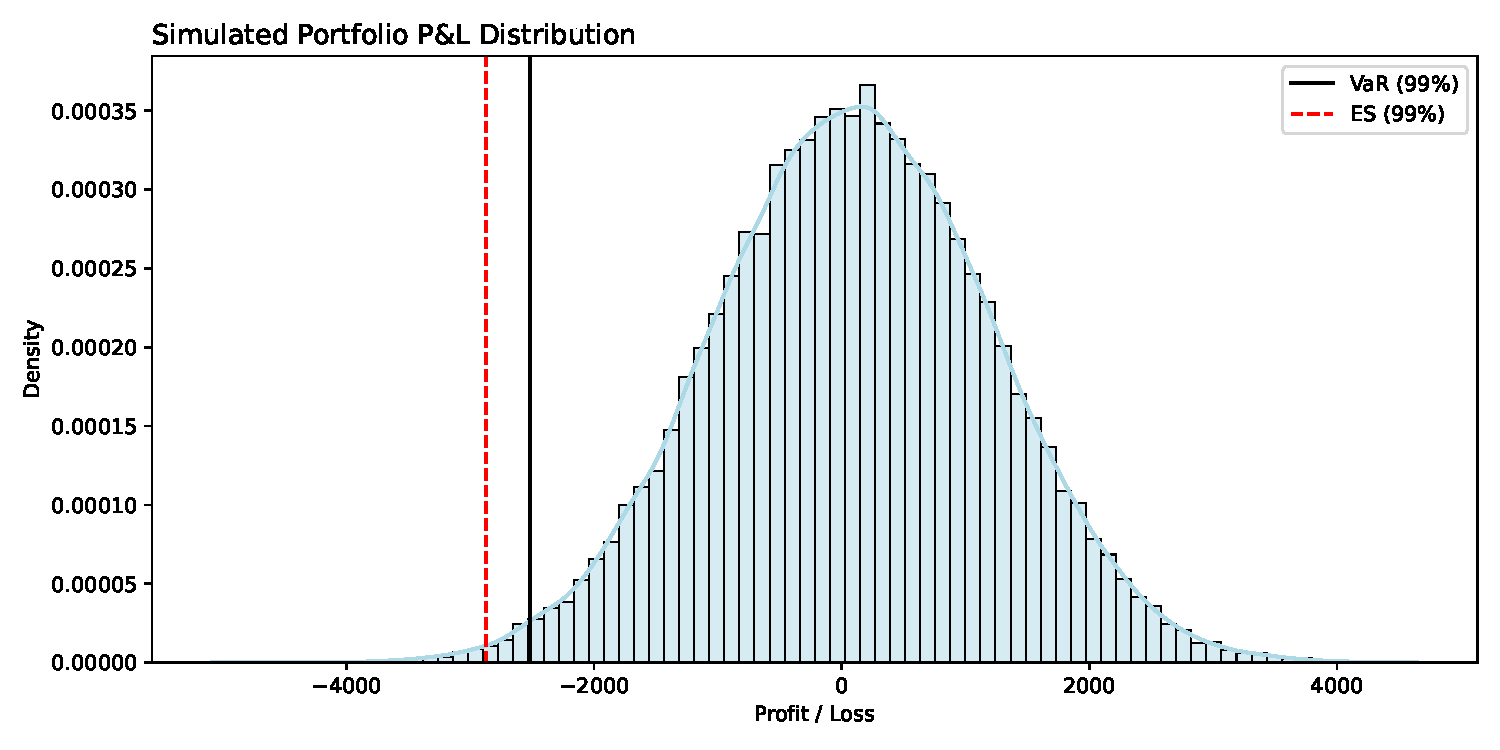
\includegraphics[width=0.8\textwidth]{figures/mc_simulation.pdf}
    \caption{Monte Carlo Simulation Results (1-Day VaR and ES)}
\end{figure}

The GARCH model using the GJR specification with skewed-t innovations also reported 42 violations, for a violation rate of 1.01\%. The Kupiec test statistic was 0.0047 (p-value: 0.9454). The Christoffersen independence test yielded a value of 0.5786 (p-value: 0.4468). The joint test statistic was 0.5833, with a p-value of 0.7470.

\begin{figure}[H]
    \centering
    \includegraphics[width=0.8\textwidth]{figures/garch_backtest.pdf}
    \caption{Backtest of GARCH VaR (GJR, skewed-t)}
\end{figure}
